\documentclass[11pt,reqno]{amsart}
\usepackage{mathptmx}
\usepackage{mathtools}
\usepackage{mathrsfs}
\usepackage[all]{xy}
\usepackage{stmaryrd}
\usepackage{fancyhdr}

\usepackage{pgf, tikz}
\usetikzlibrary{arrows, automata}

\usepackage{tikz-cd}
\usepackage{cite}
\usepackage{amsmath,amsfonts}
\usepackage{graphicx}
\usepackage{wrapfig}
\usepackage{array}
\usepackage{amsmath,amsthm,amssymb,hyperref}
\usepackage{exercise}

\usepackage{enumerate}
\usepackage{tikz}
\pagestyle{plain}
\usepackage[left=1.2in, right=1.2in, top=1in, bottom=1in]{geometry}
\usepackage{etoolbox}
\usepackage{color}
\usepackage{xcolor}
\patchcmd{\section}{\scshape}{\bfseries}{}{}
\makeatletter
\renewcommand{\@secnumfont}{\bfseries}
\makeatother
% \xyoption{all}
\thispagestyle{empty}

\DeclareMathOperator{\Hom}{Hom}
\DeclareMathOperator{\Spec}{Spec}
\DeclareMathOperator{\Spv}{Spv}
\DeclareMathOperator{\Frac}{Frac}
\DeclareMathOperator{\Img}{Img}
\DeclareMathOperator{\Ker}{Ker}
\DeclareMathOperator{\Pic}{Pic}
\DeclareMathOperator{\Jac}{Jac}
\DeclareMathOperator{\Div}{Div}
\DeclareMathOperator{\dv}{Div}
\DeclareMathOperator{\Deg}{deg}
\DeclareMathOperator{\Aut}{Aut}
\DeclareMathOperator{\CSpec}{Cspec}

\newcommand{\angles}[1]{\langle #1 \rangle}
\newcommand{\R}{\mathbb{R}}  
\newcommand{\Z}{\mathbb{Z}}
\newcommand{\N}{\mathbb{N}}
\newcommand{\Q}{\mathbb{Q}}
\newcommand{\I}{\mathbf{I}}

\newcommand{\jaiung}[1]{{\textcolor{red}{Jaiung: #1}}}
\newcommand{\youngsu}[1]{{\textcolor{blue}{Youngsu: #1}}}
\newcommand{\matt}[1]{{\textcolor{cyon}{Matt: #1}}}

% \input xy
% \xyoption{all}
\thispagestyle{empty}

%\usepackage{secdot}

\theoremstyle{definition}
\newtheorem{mydef}{\textbf{Definition}}[section]
\newtheorem{myeg}[mydef]{\textbf{Example}}
\newtheorem{conj}[mydef]{\textbf{Conjecture}}
\newtheorem*{noconj}{\textbf{Conjecture}}
\newtheorem{observ}[mydef]{\textbf{Observation}}
\newtheorem{question}[mydef]{\textbf{Question}}
\newtheorem{rmk}[mydef]{\textbf{Remark}}
\newtheorem*{que}{\textbf{Question}}
\newtheorem*{goal}{\textbf{Goal}}

\theoremstyle{plain}
\newtheorem{mythm}[mydef]{\textbf{Theorem}}
\newtheorem*{nothm}{\textbf{Theorem}}
\newtheorem*{nomainthm}{\textbf{Main Theorem}}
\newtheorem*{nothma}{\textbf{Theorem A}}
\newtheorem*{nothmb}{\textbf{Theorem B}}
\newtheorem*{nothmc}{\textbf{Theorem C}}
\newtheorem*{nothmd}{\textbf{Theorem D}}
\newtheorem*{nothme}{\textbf{Theorem E}}
\newtheorem*{nothmf}{\textbf{Theorem F}}
\newtheorem*{nothmg}{\textbf{Theorem G}}
\newtheorem{mytheorem}[mydef]{\textbf{Theorem}}
\newtheorem{lem}[mydef]{\textbf{Lemma}}
\newtheorem{pro}[mydef]{\textbf{Proposition}}
\newtheorem{claim}[mydef]{\textbf{Claim}}
\newtheorem{cor}[mydef]{\textbf{Corollary}}
\newtheorem{con}[mydef]{\textbf{Construction}}

\patchcmd{\abstract}{\scshape\abstractname}{\normalsize{\textbf{\abstractname}}}{}{}
\begin{document}

\title{On Picard groups of directed graphs}

\author{Jaiung Jun}
\address{Department of Mathematics, State University of New York at New Paltz, NY 12561, USA}
\email{junj@newpaltz.edu}

\author{Youngsu Kim}
\address{Department of Mathematics, California State University San Bernardino, San Bernardino, CA 92407}
% \curraddr{}
\email{youngsu.kim@csusb.edu}

\author{Matthew Pisano}
\address{Department of Mathematics, State University of New York at New Paltz, NY 12561, USA}
\email{pisanom1@newpaltz.edu}

%\makeatletter
%\@namedef{subjclassname@2020}{
%	\textup{2020} Mathematics Subject Classification}
%\makeatother

\subjclass[2020]{05C50, 05C76}
\keywords{Jacobian of a graph, sandpile group, critical group, chip-firing game, gluing graphs, cycle graph, Tutte
	polynomial, Tutte's rotor construction}

\maketitle

\section{Introduction}
%\begin{goal}[8/1/2022]$ $
%	\begin{enumerate}
%		\item
%		Prove/disprove: for an oriented graph $G$, one always has $\Pic(G)=\mathbb{Z} \times \Jac(G)$,
%		i.e., as a finitely generated abelian group, the rank of $\Pic(G)$ is $1$.
%		\textcolor{red}{Jaiung: we disproved this by using~\cite{wagner2000critical}.}
%		\item
%		Prove/disprove: for $C_n$, and $0 \leq m \leq n$, one can always find an orientation
%		of $C_n$ so that $\Jac(C_n)=\mathbb{Z}_m$ (with the orientation).
%		\item
%		Prove/disprove: for an oriented graph $G$, if $v_0 \in V(G)$ is a sink (or a source)
%		and $G'$ is the graph obtained by reserving the direction for all arrows adjacent
%		to $v_0$ from $G$, then $\Jac(G)=\Jac(G')$. (Note: we believe that this should be true
%		for at least some classes of graphs such as cyclic graphs.)
%		\item
%		Prove/disprove: for an oriented planar graph $G$ and its planar dual (should be defined)
%		$\hat{G}$, one has $\Jac(G)=\Jac(\hat{G})$.
%		\item
%		Prove/disprove: for oriented graphs $G_1,G_2$, let $G$ be the graph obtained by
%		gluing $G_1$ and $G_2$ along one vertex. Then $\Jac(G)=\Jac(G_1) \times \Jac(G_2)$.
%		\textcolor{red}{Jaiung: we are currently working on this (8/31)}
%	\end{enumerate}
%\end{goal}

	This project will study Chip-Firing games and how different combinations of directed and undirected edges affect its winning strategies. 
	We will focus on Research Project 11 in~\cite{glass2020chip}.
	Our plan is to pursue this for trees, cycle graphs, pseudotrees, and wheel graphs.

	% \youngsu{test}

		We explore a combinatorial game on finite graphs, called Chip-Firing Games,
	which has various connections to other areas, such as algebraic geometry, number theory and economics.
	To play the game, one first puts an integer amount of chips at each vertex. 
	Then, each vertex is allowed to borrow or lend chips from its neighbors equally as the game progresses.
	One can study chip-firing games on a graph $G$ through a finitely generated abelian group
	$\Pic(G)$ (Picard group) and its torsion subgroup $\Jac (G)$ (Jacobian) which can
	be computed by using the Laplacian matrix of $G$.

	When a graph $G$ is directed, one may extend the definition of $\Pic(G)$ and $\Jac (G)$ for undirected
	graphs by using Laplacian matrices. 
	However, computations become much more complicated. 
	For example, $\Pic(G)=\mathbb{Z}$ for any undirected tree $G$. 
	This follows from the matrix-tree theorem, which tells us that $|\Jac (G)|$ is
	the number of spanning trees of an undirected graph $G$.
	In the case of directed trees, even the rank of $\Pic(T)$ can be arbitrarily large.
	Particularly, for any natural number $n$, we can construct a tree $T_n$ such that the rank of $\Pic(T_n)$ is $n$.  \youngsu{What is $T_n$?}

	In our ongoing project, we study Picard groups and Jacobians for directed trees, cycles, and pseudotrees.
	Even in these seemingly simple cases, we find some new phenomenon. For instance, for the undirected cycle $C_n$,
	$\Jac (C_n)=\mathbb{Z}_n$, however, we prove that in the directed case, for any given $0 \le m \leq n$, one can always find an orientation of $C_n$ in such a way that $\Jac (C_n)$ is $\mathbb{Z}_m$.
	By closely examining trees and cycles, and how Picard groups and Jacobians change with (suitably defined)
	vertex and edge gluing, we obtain several results for pseudotrees.

\bigskip


\textbf{Acknowledgment}\hspace{0.1cm} This research was supported by Research and Creative Activities (RSCA) at SUNY New Paltz. We would like to thank RSCA for their support.

\section{Preliminaries}

	\subsection{Chip Firing}
		The game at the heart of this paper is the Chip-Firing game. When a game is started, each vertex on
		a graph is assigned a certain number of chips.  During play, chips can be lent or borrowed at each
		node where one or more chips are either sent or received along each outgoing edge equally.  In the
		case of a directed graph, vertices can only interact with another along an outgoing or
		bidirectional edge.  The game is won once every vertex has a positive number of chips (i.e., this
		vertex is not in debt).

	\subsection{Divisors and Equivalence Relations}
		In the study of this game a \textbf{Divisor} of a graph ($\Div(G)$) is an integer vector $v\in\mathbb{Z}^n$
		where \textit{n} is the number of vertices in the graph.  The $i^{th}$ element of the vector \textit{v}
		is the number of chips on the $i^{th}$ vertex of the graph.  Two divisors have an \textbf{equivalence relation}
		($\sim$) if one divisor can be gotten from the other by a finite series of lending or borrowing moves
		$D_1 \sim D_2 \xleftrightarrow{} (D_1 \xleftrightarrow{\text{moves}} D_2)$.  For a divisor $D$, the \textbf{equivalence class} {$[D]$}
		is the set of all divisors that are equivalent to each other, $[D] = \{D_i~|~D_i \sim D\}$.

	\subsection{The Picard Group and The Jacobian}
		The \textbf{Picard Group} of a graph $\Pic(G)$ is the set of all equivalence classes that the
		divisors of that graph can be a  part of. The \textbf{Jacobian} of a graph  $\Jac(G)$ is a subset
		of $\Pic(G)$ such that every divisor in each equivalence class has a degree of $0$, where the
		degree of a divisor $\Deg(D)$ is the sum of each of the divisor's elements.
		If a divisor is in one of the Jacobian's classes, it can be made winning after a finite series of moves.
		Here, we represent the Picard Group as $\Pic(G)=\Jac(G)\times\mathbb{Z}^n$.


\section{Gluing of directed graphs and their Jacobians}

\begin{lem}\label{proposition: gluing an arrow proposition}
Let $G$ be a directed graph. If we attach either an incoming arrow or a two-sided arrow to create another directed graph $G'$, then $\Pic(G)=\Pic(G')$.
\end{lem}
\begin{proof}
Let $\alpha$ be an arrow which is glued to $G$. Let $|V(G)|=n$. We label the vertexes of $G$ as $1,2,\dots,n$. Suppose first that $\alpha$ is incoming and $\alpha$ is glued at the vertex $n$. Let $L_G=(a_{ij})$ (resp.~$L_{G'}$) be the Laplacian matrix of $G$ (resp.~$G'$). 
Then the matrix $L_{G'}$ is of the following form.
% In this case, one can easily observe that the matrix $L_{G'}$ is of the following form:
\begin{equation}
L_{G'}=\left[\begin{array}{ccc|c|c}
a_{11}&a_{12}&\cdots &a_{1n}&0\\
a_{21}&a_{22}&\cdots &a_{2n}&0\\
\vdots & \vdots &\ddots & \vdots & \vdots \\ \hline
\vdots & \vdots & \cdots&a_n & 0\\ \hline
0&0&\cdots &-1&1\\
\end{array}\right]
\end{equation}
		By a column operation between the last two columns, we obtain the following matrix:
		\begin{equation}\label{eq: arrow adding matrix}
			\left[\begin{array}{ccc|c|c}
				a_{11}&a_{12}&\cdots &a_{1n}&0\\
				a_{21}&a_{22}&\cdots &a_{2n}&0\\
				\vdots & \vdots &\ddots & \vdots & \vdots \\ \hline
				\vdots & \vdots & \cdots&a_n & 0\\ \hline
				0&0&\cdots &0&1\\
			\end{array}\right]
		\end{equation}
		This shows that $\Pic(G)=\Pic(G')$.

		Next, suppose that $\alpha$ is a two-sided arrow. Then similar to the above, we obtain the following Laplacian matrix for $G'$:
		\begin{equation}\label{eq: eq two-sided}
			L_{G'}=\left[\begin{array}{ccc|c|c}
				a_{11}&a_{12}&\cdots &a_{1n}&0\\
				a_{21}&a_{22}&\cdots &a_{2n}&0\\
				\vdots & \vdots &\ddots & \vdots & \vdots \\ \hline
				\vdots & \vdots & \cdots&a_n+1 & -1\\ \hline
				0&0&\cdots &-1&1\\
			\end{array}\right]
		\end{equation}
		By a column operation, the matrix~\eqref{eq: eq two-sided} becomes the matrix~\eqref{eq: arrow adding matrix}.
		This shows that $\Pic(G)=\Pic(G')$.
	\end{proof}

\section{Picard groups of oriented trees}

\begin{conj}
	The Jacobian of a tree graph is always trivial. 
	It follows from the matrix-tree theorem as a tree graph only has one possible spanning tree. \textcolor{red}{[Citation Needed]}
\end{conj}

The following example shows that if we change the direction of arrows, Picard groups can change drastically.

\begin{myeg}
Consider the following directed tree:
\begin{equation}
T=\left(\begin{tikzcd}
	& 1 \arrow[d] & \\
2 \arrow[r]& 3 & 4 \arrow[l]\\
& 5 \arrow[u] &
\end{tikzcd} \right)
\end{equation}
We have
\[
L_T = \begin{bmatrix}
 1& 0& -1&0 &0 \\
 0 & 1 & -1 & 0 &0\\
 0& 0& 0& 0 &0\\
 0& 0&-1&1 & 0\\
 0& 0&-1&0 & 1
\end{bmatrix} \implies SNF(L_T)=\left[\begin{array}{c|c}
I_4 & 0 \\ \hline
0 & 0
\end{array}\right]
\]
Hence, $\Pic(T)=\mathbb{Z}$. \textcolor{red}{Jaiung; $T$ can be decomposed into $1,2,3$ and $3,4,5$. This shows that the gluing along one vertex does not work for directed graphs.} On the other hand, consider the following
\begin{equation}
T'=\left(\begin{tikzcd}
		& 1 & \\
		2 & 3 \arrow[u] \arrow[r]\arrow[l] \arrow[d]& 4 \\
		& 5  &
	\end{tikzcd} \right)
\end{equation}
We have
\[
L_T = \begin{bmatrix}
	0& 0& 0&0 &0 \\
	0 & 0 & 0 & 0 &0\\
	1& 1& 4& 1 &1\\
	0& 0&0&0 & 0\\
	0& 0&0&0 & 0
\end{bmatrix} \implies \Pic(T')=\mathbb{Z}^4.
\]
\end{myeg}

\begin{mydef}
\textcolor{red}{Jaiung: Recall terminal strong components}
\end{mydef}

\begin{pro}
		Let $T$ be a tree with any orientation. Then $\Pic(T)=\mathbb{Z}^r$, where $r$ is the number of the terminal strong components of $T$. In particular, if $T$ has no two-sided arrow, then $r$ is the number of sinks.
	\end{pro}
\begin{proof}
Note that from~\cite[Corollary 3.5]{wagner2000critical} that the rank of $\Pic(T)$ is the number of sinks of $T$.

Now, we can inductively prove this. When $T_0$ is a tree with one arrow, one can easily check that $\Pic(T_0) =\mathbb{Z}$ or $\{0\}$ (depending on the number of sinks). Suppose that $T_k$ is an oriented tree with $k$ arrows. When we add one arrow $\alpha$ to $T_k$ to construct $T_{k+1}$, there are three cases; $\alpha$ is $(1)$ incoming, $(2)$ outgoing, and $(3)$ two-sided. When $\alpha$ is either incoming or two-sided arrow, then it follows from Lemma \ref{proposition: gluing an arrow proposition} that $\Pic(T_k)=\Pic(T_{k+1})=\mathbb{Z}^r$, where $r$ is the number of sinks of $T_k$ and $T_{k+1}$, since in this case it does not increase the number of sinks.

Next, suppose that $\alpha$ is an outgoing arrow. Let's label the vertexes of $G$ as $v_1,v_2,\dots,v_n$. Suppose that the arrow $\alpha$ is attached to the vertex $v_j$. Let $L_{k}=(a_{ij})$ be the Laplacian matrix of $T_k$. Then we have the following:
\begin{equation}\label{eq: tree case}
L_{{k+1}}=\left[\begin{array}{ccccc|c|c}
a_{11}&a_{12}&\cdots& a_{1j}& \cdots&a_{1n}&0\\
a_{21}&a_{22}&\cdots& a_{2j}& \cdots&a_{2n}&0\\
\vdots & \vdots &\ddots&\vdots & \vdots&\vdots & \vdots \\
a_{j1}&a_{j2}&\cdots& a_{jj}+1 & \cdots&a_{jn}&-1\\
\vdots & \vdots & \cdots&\vdots &\vdots &\vdots & \vdots\\
a_{n1}&a_{n2}&\cdots& a_{nj} & \cdots&a_{nn}& 0\\  \hline
0&0&\cdots&\cdots &0 &0&0\\
\end{array}\right]
\end{equation}
To compute the Smith normal form, by relabeling vertices, we may assume $L_{k+1}$ is the following matrix:
\begin{equation}\label{eq: tree case2}
\left[\begin{array}{ccc|c|c}
		a_{11}&a_{12}&\cdots &a_{1n}&0\\
		a_{21}&a_{22}&\cdots &a_{2n}&0\\
		\vdots & \vdots &\ddots & \vdots & \vdots \\ \hline
		\vdots & \vdots & \cdots&a_n & 1\\ \hline
		0&0&\cdots &0&0\\
	\end{array}\right]
\end{equation}
Since $\Pic(T_k)=\mathbb{Z}^r$, there exist $P, Q \in \textrm{GL}_n(\mathbb{Z})$ such that
\begin{equation}
PL_kQ = \left[\begin{array}{c|c}
			I_{n-r} & 0 \\ \hline
	0 & 0_r
\end{array}\right]
\end{equation}
where $0_r$ is an $r\times r$ zero matrix. Consider the following block matrices of size $(n+1)\times(n+1)$:
\begin{equation}
P' = \left[\begin{array}{c|c}
	P & 0 \\ \hline
	0 & 1
\end{array}\right], \quad Q' = \left[\begin{array}{c|c}
Q & 0 \\ \hline
0 & 1
\end{array}\right]
\end{equation}
Then, we have
\begin{equation}\label{eq: matrix comp}
P'L_{k+1}Q' =  \left[\begin{array}{c|c}
	P & 0 \\ \hline
	0 & 1
\end{array}\right]  \left[\begin{array}{c|c}
L_k & e_n \\ \hline
0 & 0
\end{array}\right]\left[\begin{array}{c|c}
Q & 0 \\ \hline
0 & 1
\end{array}\right]=\left[\begin{array}{c|c}
	PL_kQ & Pe_n \\ \hline
	0 & 0
\end{array}\right]
\end{equation}

We first consider the case when $v_n$ is a sink. In particular, $T_{k+1}$ and $T_{k}$ have the same number of terminal strong components. In this case, the $n^{\textrm{th}}$ row of $L_{k+1}$ in \eqref{eq: tree case2} is the zero row. In particular, we can take $P$ so that
\begin{equation}
Pe_n=e_n
\end{equation}
Therefore, we have
\begin{equation}
P'L_{k+1}Q' = \left[\begin{array}{c|c}
	PL_kQ & Pe_n \\ \hline
	0 & 0
\end{array}\right] =\left[\begin{array}{c|c}
PL_kQ & e_n \\ \hline
0 & 0
\end{array}\right] =\left[\begin{array}{c|c|c|c}
I_{n-r} & & 0&0\\ \hline
   &0_{r-1} &0& 0\\ \hline
0 &0& 0&1\\ \hline
0 &0& 0&0\\
\end{array}\right]
\end{equation}
It follows that $\Pic(T_{k+1})=\Pic(T_k)$. Now, suppose that $v_n$ is not a sink.
\begin{equation}\label{eq: tree case3}
L_{k+1}=	\left[\begin{array}{ccc|c|c}
		a_{11}&a_{12}&\cdots &a_{1n}&0\\
		a_{21}&a_{22}&\cdots &a_{2n}&0\\
		\vdots & \vdots &\ddots & \vdots & \vdots \\ \hline
		\vdots & \vdots & \cdots&a_n & 1\\ \hline
		0&0&\cdots &0&0\\
	\end{array}\right]
\end{equation}
Note that $\textrm{rank}(L_{k+1})$ is same either we look at it over integers or rational numbers. Since $v_n$ is not a sink, the $n^{\textrm{th}}$ row of $L_k$ is not a zero row.

So, we have $\Pic(T_{k+1})=\mathbb{Z}\times \Pic(T_k)$.

\end{proof}

\begin{myeg}\label{example: oriented tree}
Consider the following oriented tree:
\[
T=\left(\begin{tikzcd}
1
	& 2 \arrow[d,swap] &  3 \arrow[d] & \\
	& 4\arrow[r,swap] \arrow[ul] & 5 \arrow[l] \arrow[u]\arrow[r,swap] & 6
\end{tikzcd}\right)
\]
The Laplacian matrix of $T$ is the following:
\[
L_T = D_T - A_T = \begin{bmatrix}
0& 0& 0& 0& 0&0 \\
0& 1&0 & 0& 0&0 \\
0& 0& 1& 0& 0&0 \\
0&0 &0 &2 &0 & 0\\
0&0 &0 &0 &3 &0 \\
0& 0& 0& 0& 0&0
\end{bmatrix} - \begin{bmatrix}
0 & 0& 0& 0& 0& 0\\
0& 0& 0&1 &0 & 0\\
0&0 &0 &0 &1 &0 \\
1& 0& 0& 0&1 &0 \\
0& 0& 1&1 &0 &1 \\
0& 0& 0& 0& 0& 0
\end{bmatrix} = \begin{bmatrix}
0&0 &0 &0 &0 &0 \\
0&1 &0 &-1 &0 &0 \\
0& 0& 1&0 &-1 &0 \\
-1& 0& 0& 2&-1 &0 \\
0&0 &-1 &-1 &3 &-1 \\
0& 0&0 &0 &0 &0
\end{bmatrix}
\]
The Smith normal form of $L_T$ is the following $6\times 6$ matrix:
\[
\left[\begin{array}{c|c}
	I_4 & 0 \\ \hline
	0 & 0_2
\end{array}\right]
\]
This shows that $\Pic(T)=\mathbb{Z}^2$.
\end{myeg}

\begin{myeg}
Consider the following oriented tree obtain from Example \ref{example: oriented tree} by gluing an outgoing arrow $\alpha$:
\[
T'=\left(\begin{tikzcd}
	1 	& 2 \arrow[d,swap] &  3 \arrow[d] & \\
	7& 4\arrow[r,swap] \arrow[ul] \arrow[l,"\alpha"] & 5 \arrow[l] \arrow[u]\arrow[r,swap] & 6
\end{tikzcd}\right)
\]
Now, we have
\[
L_{T'} = \begin{bmatrix}
	0&0 &0 &0 &0 &0 &0 \\
	0&1 &0 &-1 &0 &0 &0\\
	0& 0& 1&0 &-1 &0 &0\\
	-1& 0& 0& 3&-1 &0 &-1\\
	0&0 &-1 &-1 &3 &-1 &0\\
	0& 0&0 &0 &0 &0 & 0 \\
	0& 0&0 &0 &0 &0 & 0
\end{bmatrix}
\]
The Smith normal form of $L_{T'}$ is the following $7 \times 7$ matrix:
\[
\left[\begin{array}{c|c}
	I_4 & 0 \\ \hline
	0 & 0_3
\end{array}\right]
\]
This shows that $\Pic(T)=\mathbb{Z}^3$.
\end{myeg}

\begin{myeg}
Consider the following oriented tree obtain from Example \ref{example: oriented tree} by gluing an outgoing arrow $\alpha$:
\[
T''=\left(\begin{tikzcd}
	1
	& 2 \arrow[d,swap] &  3 \arrow[d] & 7\\
	& 4\arrow[r,swap] \arrow[ul] & 5 \arrow[l] \arrow[u]\arrow[r,swap] & 6 \arrow[u,swap,"\alpha"]
\end{tikzcd}\right)
\]
Now, we have
\[
L_{T''}=\begin{bmatrix}
	0&0 &0 &0 &0 &0 &0 \\
	0&1 &0 &-1 &0 &0 &0\\
	0& 0& 1&0 &-1 &0 &0\\
	-1& 0& 0& 2&-1 &0 &0\\
	0&0 &-1 &-1 &3 &-1 &0\\
	0& 0&0 &0 &0 &1 & -1 \\
	0& 0&0 &0 &0 &0 & 0
\end{bmatrix}
\]
The Smith normal form of $L_{T''}$ is the following $7 \times 7$ matrix:
\[
\left[\begin{array}{c|c}
	I_5 & 0  \\ \hline
	0 & 0_2
\end{array}\right]
\]
This shows that $\Pic(T'')=\mathbb{Z}^2$.
\end{myeg}


\section{Picard groups of oriented cycles}

	\subsection{Representing Single Term Jacobians}
		\begin{conj}
			Let $C_n$ be the cycle graph with $n$ vertices. For each $k \leq n$, there exists an orientation of $C_n$
			such that $\Jac(C_n)$ (with that orientation) is $\mathbb{Z}_k$.
		\end{conj}

		The following examples confirms the conjecture for the class of $C_3$.

		\begin{myeg}
		\begin{figure}[h!]
		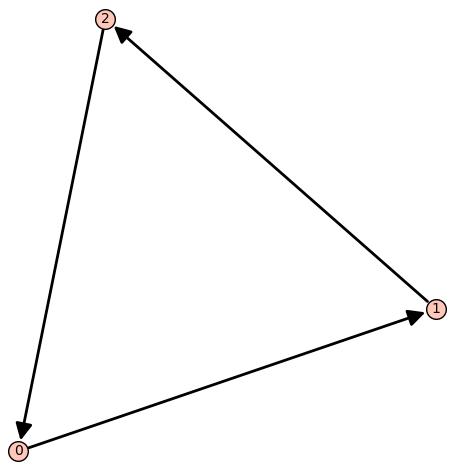
\includegraphics[width=0.3\textwidth]{3-vertices1.PNG}
		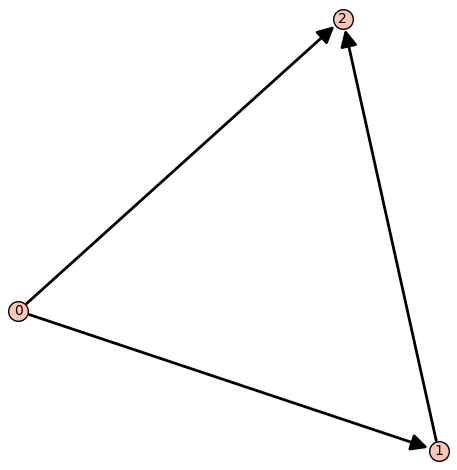
\includegraphics[width=0.3\textwidth]{3-vertices2.PNG}
		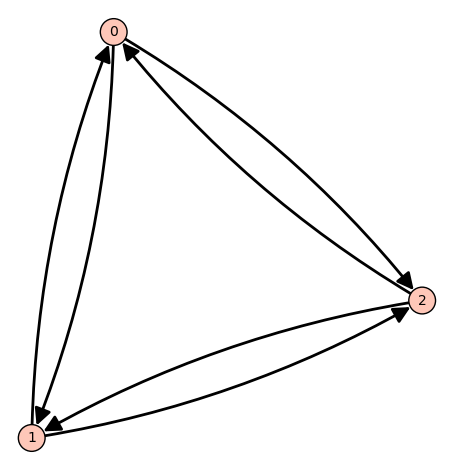
\includegraphics[width=0.3\textwidth]{3-vertices3.PNG}
		\caption{Digrphs with Jacobians $0, \mathbb{Z}_2$, and $\mathbb{Z}_3$}
		\end{figure}
			% cycle = Graph.cycle(3)
			% cycle.setEdgeState(0, 1, 2)
			% cycle.setEdgeState(1, 2, 2)
			% cycle.setEdgeState(2, 0, 2)
			% Trivial

			% cycle = Graph.cycle(3)
			% cycle.setEdgeState(0, 1, 1)
			% cycle.setEdgeState(1, 2, 2)
			% cycle.setEdgeState(2, 0, 2)
			% Z_2

			% cycle = Graph.cycle(3)
			% cycle.setEdgeState(0, 1, 0)
			% cycle.setEdgeState(1, 2, 0)
			% cycle.setEdgeState(2, 0, 0)
			% Z_3
		\end{myeg}

		The number of paths in the cycle graph also plays a role in if it can represent all single term Jacobians up
		to $\mathbb{Z}_n$.
		
		\begin{rmk}
			Let $M$ be an $m$ by $n$ matrix, 
			and let $I_k(M)$ denote the ideal generated by $k \times k$ minors of $M$, 
			where $I_k(M) = 0$ if $k > \min\{m,n\}$ and $I_k = (1)$ if $k \le 0$. 
			For a matrix $N = \left( \begin{array}{c|c}
				M & 0 \\
				\hline
				0 & 1
			\end{array} \right)$ and for any $k$, $I_k(M) = I_{k+1}(N)$, and the cokernels of $M$ and $N$ are isomorphic. 
		\end{rmk}

		\begin{lem}
		Let $C_n$ be a directed cycle graph on $n$ vertices. If not every edge is bidirectional, there is a directed cycle graph $C_{n+1}$ such that $\Pic (C_n) \cong \Pic (C_{n+1})$. 
		\end{lem}

		\begin{proof}
			Let $D_{C_n} = (d_{ij})$. Since not every edge is bidirectional, there exists $i$ such that $d_{i,i} = 0$ or $1$.
			Without loss of generality, we may assume $i = n$ so that the nearby vertices are $V_{n-1}$ and $V_1$.
			If $d_{n,n} = 0$, 
			then the Laplacian matric of $C_n$ is the following. 
			$$
			L_{C_n} = 
			\begin{bmatrix}
				l + 1 & -l & 0 & \cdots & 0 & -1 \\
				\vdots & \vdots & \vdots & \cdots \\
				0 & \cdots & 0 & -k & k+1 & -1 \\
				0 & \cdots & 0 & 0 & 0 & 0 
			\end{bmatrix}$$
			where $l, k \in \{ 0, 1 \}$. 
			We define $C_{n+1}$ extending $C_n$ as follows. 
			Add a vertex $V_{n+1}$ to $C_n$, replace the edge $E_{1\to n}$ by $E_{1 \to n+1}$, and add a new edge $E_{n \to n+1}$. 
			Pictorially, we have the following
			\[
				C_n: \left( \cdots \begin{tikzcd}
					V_{n-1} \arrow[r] & V_n & V_1 \arrow[l] 
				\end{tikzcd} \cdots \right)
				\longrightarrow
				C_{n+1}: \left( \cdots \begin{tikzcd}
					V_{n-1} \arrow[r] & V_n \arrow[r] & V_{n+1} &  V_1 \arrow[l] 
				\end{tikzcd} \cdots \right).
			\]
			Now, one has the following equivalence of matrices.
			\begin{align}
			L_{C_{n+1}} &= 
			\begin{bmatrix} 
				l + 1 & -l & 0 & \cdots & 0 & -1 \\
				\vdots & \vdots & \vdots & \cdots \\
				0 & \cdots & -k & k+1 & -1 &0 \\
				0 & \cdots & 0 & 0 & 1 & -1 \\
				0 & \cdots & 0 & 0 & 0 & 0 
			\end{bmatrix} 
			\stackrel{R_{1} \to R_1 + R_{n-1}}\sim 
			\begin{bmatrix} 
				l + 1 & -l & 0 & \cdots & -1 & 0 \\
				\vdots & \vdots & \vdots & \cdots \\
				0 & \cdots & -k & k+1 & -1 &0 \\
				0 & \cdots & 0 & 0 & 1 & -1 \\
				0 & \cdots & 0 & 0 & 0 & 0 
			\end{bmatrix} \\
			&\stackrel{C_{n-1} \to C_{n-1} + C_{n}}\sim
			\begin{bmatrix} 
				l + 1 & -l & 0 & \cdots & -1 & 0 \\
				\vdots & \vdots & \vdots & \cdots \\
				0 & \cdots & -k & k+1 & -1 &0 \\
				0 & \cdots & 0 & 0 & 0 & -1 \\
				0 & \cdots & 0 & 0 & 0 & 0 
			\end{bmatrix}
			\sim
			\begin{bmatrix} 
				l + 1 & -l & 0 & \cdots & -1 & 0 \\
				\vdots & \vdots & \vdots & \cdots \\
				0 & \cdots & -k & k+1 & -1 &0 \\
				0 & \cdots & 0 & 0 & 0 & 0 \\
				0 & \cdots & 0 & 0 & 0 & 1 
			\end{bmatrix}\\
			&=
			\left( \begin{array}{c|c}
				L_C & 0 \\
				\hline
				0 & 1
			\end{array} \right).
			\end{align}
			Then the remark above proves the claim.

			Now suppose $d_{n,n} = 1$. Without loss of generality, we may assume the vertex $V_n$ has an one outgoing edge to $V_1$. 
			There are two cases, depending on the exsitence of $E_{1\to n}$.
			The Laplacian of these two graphs are equivlent. 
			$$
			L_{C_n} = \begin{bmatrix}
				l  & -l & 0 & \cdots & 0 & 0 \\
				\vdots & \vdots & \vdots & \cdots \\
				0 & \cdots & 0 & -k & k+1 & -1 \\
				-1 & \cdots & 0 & 0 & 0 & 1 
			\end{bmatrix}
			\stackrel{R_{1}\to R_1  - R_n}\sim
			\begin{bmatrix}
				l+1  & -l & 0 & \cdots & 0 & -1 \\
				\vdots & \vdots & \vdots & \cdots \\
				0 & \cdots & 0 & -k & k+1 & -1 \\
				-1 & \cdots & 0 & 0 & 0 & 1 
			\end{bmatrix},
			$$
			where $l, k \in \{ 0, 1 \}$. 
			Therefore, we may assume that $L_{C_n}$ the first matrix.
			We define $C_{n+1}$ extending $C_n$ as follows. 
			Add a vertex $V_{n+1}$ to $C_n$, 
			replace the edge $E_{n \to 1}$ by $E_{n+1 \to 1}$, and 
			add a new edge $E_{n \to n+1}$. 
			Pictorially, we have the following
			\[
				C_n: \left( \cdots \begin{tikzcd}
					V_{n-1} \arrow[r] & V_n \arrow[r] & V_1 
				\end{tikzcd} \cdots \right)
				\longrightarrow
				C_{n+1}: \left( \cdots \begin{tikzcd}
					V_{n-1} \arrow[r] & V_n \arrow[r] & V_{n+1} \arrow[r] & V_1 
				\end{tikzcd} \cdots \right).
			\]
			Then we have the following equivalence of matrices.
			\begin{align}
			L_{C_{n+1}} &= 
			\begin{bmatrix} 
				l  & -l & 0 & \cdots & 0 & 0 & 0 \\
				\vdots & \vdots & \vdots & \cdots \\
				0 & \cdots & 0 & -k & k+1 & -1 & 0  \\
				0 & \cdots & 0 & 0 & 0 & 1 & -1 \\ 
				-1 & \cdots & 0 & 0 & 0 & 0 & 1 
			\end{bmatrix} \stackrel{R_{n-1}\leftrightarrow R_{n}}{\sim}
			\begin{bmatrix} 
				l  & -l & 0 & \cdots & 0 & 0 & 0 \\
				\vdots & \vdots & \vdots & \cdots \\
				0 & \cdots & 0 & -k & k+1 & -1 & 0  \\
				-1 & \cdots & 0 & 0 & 0 & 0 & 1 \\
				0 & \cdots & 0 & 0 & 0 & 1 & -1 
			\end{bmatrix} \\ 
			&\stackrel{R_{n-1} \to R_{n-1} + R_{n}}\sim 
			\begin{bmatrix} 
				l  & -l & 0 & \cdots & 0 & 0 & 0 \\
				\vdots & \vdots & \vdots & \cdots \\
				0 & \cdots & 0 & -k & k+1 & -1 & 0  \\
				-1 & \cdots & 0 & 0 & 0 & 1 & 0 \\ 
				0 & \cdots & 0 & 0 & 0 & 1 & -1 \\ 
			\end{bmatrix}
			\stackrel{C_{n-1} \to C_{n-1} - C_{n}}\sim 
			\begin{bmatrix} 
				l  & -l & 0 & \cdots & 0 & 0 & 0 \\
				\vdots & \vdots & \vdots & \cdots \\
				0 & \cdots & 0 & -k & k+1 & -1 & 0  \\
				-1 & \cdots & 0 & 0 & 0 & 1 & 0 \\ 
				0 & \cdots & 0 & 0 & 0 & 0 & -1 \\ 
			\end{bmatrix} \\
			&\sim 
			\left( \begin{array}{c|c}
				L_C & 0 \\
				\hline
				0 & 1
			\end{array} \right).
			\end{align}
			Again, the remark above proves the claim.
		\end{proof}

		\begin{lem}
			For any $n \ge 4$ and any $m \in \{ n-1, n \}$, there exists a direct graph $C_n$ on $n$ vertices such that $\Jac (C_n) = \Z_m$. 
		\end{lem}

		\begin{proof}
			The directed cyclic graph $C_n$ with all bidirectional edges has $\Pic (C_n) \cong \Z_n$. 
			We claim that a directed cyclic graph $C_n$ such that 
			\[
			C_n: \left( \cdots \begin{tikzcd}
				V_n \arrow[r] & V_1 & V_2 \arrow[l] & V_3 \arrow[l]
			\end{tikzcd} \cdots \right)
			\]
			and all other edges are bidirection has the Picard group $Z_{n-1}$. 
			We have the following equivalnec of matrices.
			\begin{align}
			L_{C_n} &= \begin{bmatrix}
				0 & 0 & 0 & 0 & 0 & 0 & 0 & 0   \\
				-1 & 1 & 0 & \cdots & 0 & 0 & 0 & 0  \\
				0 & -1 & 2 & -1 & \cdots & 0 & 0 & 0 \\
				0 & 0 & -1 & 2 & -1 & \cdots & 0 & 0  \\
				\vdots \\
				-1 & 0 & 0 & 0 & 0 & \cdots & -1 & 2 \\
			\end{bmatrix}
			\stackrel{R_{n} \to R_{n} - R_{2}}\sim 
			\begin{bmatrix}
				0 & 0 & 0 & 0 & 0 & 0 & 0 & 0   \\
				-1 & 1 & 0 & \cdots & 0 & 0 & 0 & 0  \\
				0 & -1 & 2 & -1 & \cdots & 0 & 0 & 0 \\
				0 & 0 & -1 & 2 & -1 & \cdots & 0 & 0  \\
				\vdots \\
				0 & -1 & 0 & 0 & 0 & \cdots & -1 & 2 \\
			\end{bmatrix}\\
			&\stackrel{C_2 \to C_2+C_1}\sim 
			\begin{bmatrix}
				0 & 0 & 0 & 0 & 0 & 0 & 0 & 0   \\
				-1 & 0 & 0 & \cdots & 0 & 0 & 0 & 0 \\
				0 & -1 & 2 & -1 & \cdots & 0 & 0 & 0 \\
				0 & 0 & -1 & 2 & -1 & \cdots & 0 & 0  \\
				\vdots \\
				0 & -1 & 0 & 0 & 0 & \cdots & -1 & 2 \\
			\end{bmatrix}
			\sim 
			\begin{bmatrix}
				1 & 0 & 0 & \cdots & 0 & 0 & 0 & 0 \\
				0 & 0 & 0 & 0 & 0 & 0 & 0 & 0   \\
				0 & -1 & 2 & -1 & \cdots & 0 & 0 & 0 \\
				0 & 0 & -1 & 2 & -1 & \cdots & 0 & 0  \\
				\vdots \\
				0 & -1 & 0 & 0 & 0 & \cdots & -1 & 2 \\
			\end{bmatrix}\\
			&\sim \begin{bmatrix}
				1 & 0 & 0 & \cdots & 0 & 0 & 0 & 0 \\
				0 & 2 & -1 & 0 & 0 & 0 & 0 & -1   \\
				0 & -1 & 2 & -1 & \cdots & 0 & 0 & 0 \\
				0 & 0 & -1 & 2 & -1 & \cdots & 0 & 0  \\
				\vdots \\
				0 & -1 & 0 & 0 & 0 & \cdots & -1 & 2 \\
			\end{bmatrix} \tag{See the remark below for the last equivalance}
			\end{align}
			Now the $n-1 \times n-1$ bottom right submatrix is that of $C_{n-1}$ with all bidirecional edges and the remark above proves the claim.
		\end{proof}

		\begin{rmk}
			For $n \ge 3$, the Laplacian of $C_n$ each of its edge is bidirecional, the Laplacian of $C_n$ is of the form
			$$
			L = 
			\begin{bmatrix}
				2 & -1 & 0 & 0 & 0 & 0 & -1   \\
				-1 & 2 & -1 & \cdots & 0 & 0 & 0 \\
				0 & -1 & 2 & -1 & \cdots & 0 & 0  \\
				\vdots \\
				-1 & 0 & 0 & 0 & \cdots & -1 & 2 \\
			\end{bmatrix}
			$$
			Since $[1 \cdots 1] L = 0$, 
			the first row is a $\Z$-linear combination of the next $n-1$ rows. 
			This justifies the last equivalance in the proof above.  
		\end{rmk}

		\begin{proof}[Proof of the Conjecture]
		We induct on the number of edges. The base case is when $n = 3$ which is our example. 
		For $n > 3$, by the lemma above, have have a directed graph $C_n$ with $\Jac(C_n) = n, n-1$. 
		Now the rest follows from the previous lemma. 
		``This needs to be argued more carefully using maps between the set of the Jacobians for $C_n$ except for one.''
		\end{proof}
			
		\begin{conj}
			For any cycle graph $C_n$, the orientation with no paths always has a Jacobian of $\mathbb{Z}_n$.
			Either of the single path orientations have a trivial Jacobian.
			The set of all orientations with two paths always contains all single invariant factors
			$\mathbb{Z}_2\dots\mathbb{Z}_n$.  For all graphs at least up to $C_{10}$ and likely well beyond that
			point, the sets that contain all other paths do not contain all of the single invariant factors.
		\end{conj}

		It should be noted that for four paths and upward, the sets that contain these paths often also contain
		Jacobians of $\mathbb{Z}_3$ and $\mathbb{Z}_4$.  The number of each of these increases with the size of the
		graph, so it is possible that these sets will contain all of the single invariant factors for very
		large cycle graphs.

	\subsection{Describing Two Path Cycle Graphs}
		Here, a \textit{path} represents a region of a cycle graph in which all arrows are oriented in a single
		direction or are bidirectional.  In graphs with exactly two of these paths, a consistent pattern arises
		that allows for the rapid calculation of the Jacobian in only $O(n)$ time compared to the $O(n^4)$ time
		that calculating the smith normal form takes. This pattern relies on calculating the number
		of bidirectional arrows between these two paths on one side.

		\begin{conj}
			For any given cycle graph, $\Jac(G)=\mathbb{Z}_{x-2}$, where $x$ is the number of
			bidirectional edges clockwise of the counter-clockwise path and counter-clockwise of the clockwise path.
		\end{conj}
		\textcolor{green}{Matthew: For proof, perhaps see above}

	\subsection{Representing The Rank of the Picard Group for Cycle Graphs}
		The following example shows that the rank of $\Pic(C_n)$ (with an orientation) does not have to be $1$;
		this directly follows from~\cite[Corollary 3.5]{wagner2000critical}.

		\begin{myeg}
			%cycle = Graph.cycle(9)
			%cycle.setEdgeState(0, 1, 0)
			%cycle.setEdgeState(1, 2, 1)
			%cycle.setEdgeState(2, 3, 1)
			%cycle.setEdgeState(3, 4, 2)
			%cycle.setEdgeState(4, 5, 2)
			%cycle.setEdgeState(5, 6, 1)
			%cycle.setEdgeState(6, 7, 1)
			%cycle.setEdgeState(7, 8, 2)
			%cycle.setEdgeState(8, 0, 2)
			%Rank(Pic(G)) = 2: 2 terminal strong components
		\end{myeg}

		$\Pic(G)$ is often in the form $\mathbb{Z}_1 \times \dots \times \mathbb{Z}_n \times \mathbb{Z}^m$ where $m$ is
		the rank of the picard group.  A terminal strong component describes itself well.  It is a terminal component,
		meaning that its only connections are edges directed into it.  It is also strongly connected, meaning that every
		vertex in the component has at least one path to all other components.  For cycle graphs and trees, the number
		of these terminal strong components is exactly equal to $Rank(\Pic(G))$.

		\begin{proof}
			The $Rank(\Pic(G))$ comes directly from the number of all zero rows of the Smith Normal Form of the laplacian of
			$G$.  Terminal strong components are either already zero rows (in the case of a single sink) or there
			exists a series of row and column operations that, when preformed on the laplacian result in a row of all
			zeroes.
		\end{proof}

	\begin{lem}
		Let $C_n$ be the cycle graph with $n$ vertices. Consider the equi-orientation of $C_n$.
		Then $\Pic(C_n)=\mathbb{Z}$.
	\end{lem}
	\begin{proof}
		In this case $C_n$ will always have a laplacian with a diagonal of $1$ and a diagonal of $-1$
		above or below it depending on the orientation, with another $-1$ in the top right or bottom left corner
		where $V_0$ connects $V_{n-1}$.  Turing this laplacian into a smith normal form of all $1$s is as simple as
		cascading additions from the first row in a counter-clockwise case and the last row in the clockwise case.
		This will result in a diagonal of ones with the first or last column made up of mostly $-1$.  From here
		all that needs to be done is to eliminate these with the first or last row.  Since each equi-oriented $C_n$
		will follow this pattern, this algorithm will prove $\Pic(C_n)=\mathbb{Z}$ for all $C_n$.
	\end{proof}

\section{Picard groups of oriented pseudotrees}

	\textcolor{red}{Jaiung: here we study how Picard groups change when we glue two directed graphs along one vertex or
		connect two graphs along one arrow. If we are lucky this should provide a way to compute Picard groups for
		pseudotrees by using the tree case and the cycle case in the previous sections.}

\section{Picard groups of oriented wheel graphs}

	\textcolor{red}{Jaiung: the following conjecture should generalize the results in \cite{biggs1999chip}.}

	\subsection{Patterns in The Jacobian}
		For wheel graphs, we looked for patterns that arose within the invariant factors of the Jacobian as
		a general formula was not immediately obvious.  For this strategy, we broke the edges of the wheel graph into
		their two most obvious groups, those belonging to the rim of the wheel and those of the spokes.  By orienting
		all the edges of either group the same way and trying all nine combinations, we noticed a well-defined pattern
		for each as the size of the wheel graph changed.  These patterns fell into four distinct groups.

		\begin{enumerate}
			\item When the spoke edges all pointed towards the axel and the rim was not bidirectional, or when
				the spoke edges were bidirectional, but the rim was not then a graph of size $n$ had a
				Jacobian of $\mathbb{Z}_{2^(n-1)-1}$.
			\item When the spoke edges all pointed away from the axel and the rim was not bidirectional,
				a graph of size $n$ had a Jacobian of $\mathbb{Z}_{n-1}$.
			\item When the spoke edges point away from the axel and the rim was bidirectional and a graph of size
				$n$ had a Jacobian of $\mathbb{Z}_{n-1} \times \mathbb{Z}_{n-1}$ when $n$ was even
				and $Z_{\frac{n-1}{2}} x Z_{(n-1) \times 2}$ when $n$ was odd.
			\item When all edges were bidirectional or when the spoke direction was towards the axel and
				the rim was bidirectional, a graph of size $n$ had a Jacobian of
				$\mathbb{Z}_{\alpha\phi^{n}} \times \mathbb{Z}_{5\alpha\phi^{n}}$ when the size
				was odd where $\alpha \approxeq 0.27555$ and $\mathbb{Z}_{\beta\phi^{n}} \times \mathbb{Z}_{\beta\phi^{n}}$
				when the size was even where $\beta \approxeq 0.618035$. In both of these patterns,
				$\phi$ represents the golden ratio.
		\end{enumerate}

\section{Picard groups of oriented multipartite graphs}
	For our purposes, a multipartite graph is a graph whos vertices can be partitioned between several independent
	groups, arranged in a linear order.  Vertices have no connections to members of their own group, but are strongly
	connected to all vertices of their two adjacent groups.

	The structure of the graphs that we investigate are intentionally designed to resemble artificial neural networks.
	To further facilitate this comparison, we direct all edges \textit{forward} such that, after numbering the groupings
	of these vertices in some order, edges always point towards the next highest numbered grouping.

	We were able to find notable patterns in both a \textit{Perceptron} style model with two layers and a
	\textit{Hidden Layer} model with three layers.

	\subsection{Picard groups for two layers}
		For two layers in the form of $f \rightarrow s$ where $f$ and $s$ are the number of nodes in the first and
		second layers, respectively, $\Pic(G) = \mathbb{Z}_{s}^{f-1} \times \mathbb{Z}^s$.

	\subsection{Picard groups for three layers}
		For three layers in the form of $f \rightarrow s \rightarrow t$ where $f$, $s$, and $t$ are the number of nodes
		in the first, second, and third layers, respectively the Picard group is significantly more complex.

		\begin{enumerate}
			\item When $s$ is odd, $s$ is not a factor of $t$ and $f <= s$,
				$\Pic(G) = Z_{t}^{s-f-1} \times Z_{s \times t}^{f} \times Z^t$
		\end{enumerate}

%if t is odd:
%    if s is odd:
%        if s is not a factor of t:
%            if f <= s:
%                (s-f-1)Z_(t) x (f)Z_(s*t) x Z^t
%            else:
%                (f-s+1)Z_s x (s-1)Z_(s*t) x Z^t
%        else:
%            (f-1)Z_s x Z_t x Z_(s*t) x Z^t
%    else:
%        if f <= s:
%            (s-f-1)Z_(t) x (f)Z_(s*t) x Z^t
%        else:
%            (f-s+1)Z_s x (s-1)Z_(s*t) x Z^t
%
%else:
%    if s is odd:
%        if s is not a factor of t:
%            if f <= s:
%                (s-f-1)Z_(t) x (f)Z_(s*t) x Z^t
%            else:
%                (f-s+1)Z_s x (s-1)Z_(s*t) x Z^t
%        else:
%            (f-1)Z_s x Z_t x Z_(s*t) x Z^t
%    else:
%        if s is a factor of t:
%            (f-1)Z_s x Z_t x Z_(s*t) x Z^t
%        else:
%            (f-1)Z_2 x (s-f-1)Z_t x (f-1)Z_(s*t/2) x Z_(s*t) x Z^t%


\section{Experimental Results}

	\subsection{Calculations for two path cycle graphs}
		We have proven this completely for cycle graphs up to $C_{80}$ when using two continuous paths without
		any bidirectional arrows separating them on the other size.  This has also held true for many other
		arbitrary orientations that still meet the two-path definition.
\bibliography{Jacobian}
\bibliographystyle{alpha}

\end{document}